\documentclass{beamer}
\usepackage{beamerthemeshadow}

%\documentclass{article}
%\usepackage{beamerarticle}
%\usepackage{graphicx}

\usepackage{verbatim}
\usepackage{lastpage}
\usepackage{xcolor}
\usepackage{pgf}
\usepackage{colortbl}

\newcommand{\bi}{\begin{itemize}}
\newcommand{\ei}{\end{itemize}}
\newcommand{\be}{\begin{enumerate}}
\newcommand{\ee}{\end{enumerate}}
\newcommand{\bd}{\begin{description}}
\newcommand{\ed}{\end{description}}
\newcommand{\prbf}[1]{\textbf{#1}}
\newcommand{\prit}[1]{\textit{#1}}
\newcommand{\beq}{\begin{equation}}
\newcommand{\eeq}{\end{equation}}
\newcommand{\bdm}{\begin{displaymath}}
\newcommand{\edm}{\end{displaymath}}

\newcommand{\ft}[1]{
  \frametitle{\begin{tabular}{p{4.2in}r} \textcolor{white}{#1} & \small{\insertframenumber / \inserttotalframenumber} \end{tabular}}
  %\frametitle{#1}
  \setbeamercovered{transparent=18}
}

\newcommand{\stepinv}{\setbeamercovered{invisible}}
\newcommand{\stopinv}{\setbeamercovered{transparent=18}}
\newcommand{\uncoverinv}[1]
{
  \setbeamercovered{invisible}
  \uncover<+->{#1}
  \setbeamercovered{transparent=18}
}
\newcommand{\ans}[1]{\textcolor{blue}{#1}}
\newcommand{\ansinv}[1]
{
  \setbeamercovered{invisible}
  \uncover<+->{\textcolor{blue}{#1}}
  \setbeamercovered{transparent=18}
}
\newcommand{\setinv}{\setbeamercovered{invisible}}
\newcommand{\setvis}{\setbeamercovered{transparent=18}}
\newcommand{\centerpic}[2]
{
  \begin{center}
  \includegraphics[#1]{#2}
  \end{center}
}
\newcommand{\h}[1]{\hat{#1}}
\newcommand{\ds}{\displaystyle}

%\definecolor{light}{rgb}{0.17,0.55,0.35}
\newcommand{\hl}[1]{\alt<#1>{\rowcolor{light}\hspace*{-2.1pt}} {\hspace*{-2.1pt}} }

\definecolor{mycolor}{rgb}{0.17,0.55,0.35}
\usecolortheme[named=mycolor]{structure}

\title[Expectational Shocks in the New Keynesian Model]{Learning with Expectational Shocks in the New Keynesian Model}
\author[James Murray, University of Wisconsin - La Crosse]{James Murray\\Department of Economics\\University of Wisconsin - La Crosse}
\date{Friday, March 19, 2010}

\begin{document}

\frame{\titlepage}
%\maketitle
\setcounter{framenumber}{0}

\section{Introduction}
\subsection{Purpose}

\frame
{
  \ft{Purpose}
  \be
  \item How much of macroeconomic volatility in post-war U.S. is explained by...
    \bi
    \item traditional structural shocks (natural rate shock, cost shock, monetary policy shock),
    \item and shocks to judgment (aka expectational shocks)?
    \ei
  \item How much of judgment is explained by...
    \bi
    \item actual events (i.e. current structural shocks),
    \item and expectational shocks?
    \ei
  \ee
}

\subsection{Framework}
\frame
{
  \ft{Framework}
  \bi
  \item Examine predictions using an estimated three equation New Keynesian model (Woodford [2003]).
  \item Replace rational expectations with least-squares learning.
  \item Actual expectations = Least-squares forecast + Judgment.
  \ei
}

\subsection{Expectations}
\frame
{
  \ft{Learning}
  \bi
  \item Oraphanides and Williams (JEDC, 2005): Monetary authority was optimizing, but misinformed.
  \item Primiceri (QJE, 2006): Monetary authority misinformed, expectations improved with time.
  \item Milani (JME, 2007): Agents learn, little evidence of difference in policy parameters.
  \item Milani (2008): Time varying expectations explains time-varying volatility.
  \item Bullard and Singh (2007): bad luck + Bayesian learning.
  \ei
}

\frame
{
  \ft{Judgment}
  \bi
  \item Svensson (2005), Reifschneider, Stockton, and Wilcox (1997): judgment essential for central banking policy.
  \item Bullard, Evans, Honkapohja (2008), (2010): exuberance equilibria.
  \item Missing: empirical evaluation.
  \ei
  
}

\section{Framework}
\subsection{New Keynesian Model}
\frame
{
  \ft{New Keynesian Model}
  \bi
  \item Consumer behavior:
    \bi
    \item Choose consumption and labor to maximize utility.
    \item Habit formation: utility on consumption depends on past consumption.
    \ei
  \item Producer behavior:
    \bi
    \item Intermediate goods are produced with labor in monopolistically competitive markets.
    \item Intermediate goods subject to Calvo (1983) price friction.
    \item Price indexation: when not re-optimizing prices, price can adjust according to past inflation.
    \ei
  \item Taylor (1993) type monetary policy:
    \bi
    \item Nominal interest rate responds to inflation, expected future output gap, and past interest rate.
    \ei
  \ei
}

\frame
{
  \ft{Optimal Consumer Behavior}
  \uncover{\bdm \begin{array}{c} 
      \tilde{\lambda}_{t} = E_t \tilde{\lambda}_{t+1} + \h{r}_t - E_t \pi_{t+1} - r_t^n, \\ \\
      \tilde{\lambda}_t = \frac{1}{ (1-\beta \eta)(1-\eta)}\left[ \beta \eta  E_t \tilde{y}_{t+1} - (1+\beta \eta^2) \tilde{y}_t + \eta \tilde{y}_{t-1} \right] 
      \end{array}
      \edm}
  \bi
  \item Variables:
    \bi
    \item $\tilde{\lambda}_{t}$: marginal utility of income.
    \item $\tilde{y}_t$: output gap.
    \item $\h{r}_t$: nominal interest rate.
    \item $\pi_{t}$: inflation.
    \item $r_t^n$: ``natural rate'' shock, deviation of interest rate from flexible price outcome.
    \ei
  \item Parameters:
    \bi
    \item $\eta \in [0,1)$: degree of habit formation.
    \item $\beta \in (0,1)$: discount rate.
    \ei
  \ei
}

\frame
{
  \ft{Producer Behavior}
  \bi
  \item Phillips curve:
  \uncover{\bdm \pi_t = \frac{1}{1+\beta \gamma} \left[ \gamma \pi_{t-1} + \beta E_t \pi_{t+1} + \kappa (\tilde{y}_t - \mu \tilde{\lambda}_t) + u_t\right] \edm}
  \item Cost push shock: $u_t$.
  \item Parameters:
    \bi
    \item $\gamma \in [0,1)$: degree of price indexation. 
    \item $\kappa \in (0,\infty)$: reduced form parameter inversely related to degree of price flexibility.
    \ei
  \ei
}

\frame
{
  \ft{Monetary policy}
  \bi
  \item Nominal interest rate responds to expected output gap and inflation:
  \bdm \h{r}_t = \rho_r \h{r}_{t-1} + (1-\rho_r) \left(\psi_{\pi} E_t \pi_{t+1} + \psi_y E_t \tilde{y}_{t+1} \right) + \epsilon_{r,t} \edm
  \item Monetary policy shock: $\epsilon_{r,t}$.
    \bi
    \item $\psi_{\pi} \in (0,\infty)$: feedback on inflation.
    \item $\psi_{y} \in (0,\infty)$: feedback on output.
    \item $\rho_r \in (0,1)$: smoothing parameter.
    \ei
  \ei
}

\frame
{
  \ft{Structural Shocks}
  \bi
  \item Natural interest rate shock:
  \uncover{\bdm r_t^n = \rho_n r_{t-1}^n + \epsilon_{n,t} \edm}
  \item Cost push shock:
  \uncover{\bdm u_t = \rho_u u_{t-1} + \epsilon_{u,t} \edm}
  \item Monetary policy shock, $\epsilon_{r,t}$ is not autoregressive.
  \ei
}

\subsection{Expectations}
\frame
{
  \ft{Learning}
  \bi
  \item Log-linearized New Keynesian model has the structural form:
  \bdm \Omega_{0} x_t = \Omega_{1} x_{t-1} + \Omega_{2} x_{t+1}^e + \Omega_{3} x_{t+2}^e + \Psi z_t \edm
  \vspace*{-1pc}
  \item All observable by the agents: $x_t = [\tilde{y}_t~ \pi_t~ \h{r}_t]$
  \item Shocks not observable to agents that learn: $z_t = [r_t^n~ u_t~ \epsilon_{r,t}]'$
  \item Rational expectations solution:
  \bdm E_t x_{t+1} = G x_{t} + H z_t \edm
  \vspace*{-1pc}
  \item Agents estimate $G$ by constant gain least squares.
    \bi
    \item Regressors: constant, first lag of $x_t$.
    \item Constant learning gain, $g$, measures degree to which expectations are adaptive.
    \ei
  \ei
}

\frame
{
  \ft{Judgment}
  Judgment, $\eta_t$, is possibly informed by current structural shocks, and subject to is own shock:
    \bdm \begin{array}{c} \ds \eta_t = \phi_0 + \Phi z_t + \zeta_t, \\ [1pc]
      \ds \zeta_{y,t} = \rho_{\zeta,y} \zeta_{y,t-1} + \xi_{y,t}, \\ [1pc]
      \ds \zeta_{\pi,t} = \rho_{\zeta,\pi} \zeta_{\pi,t-1} + \xi_{\pi,t},
    \end{array} \edm
  Notation:
    \bi
    \item $\eta_t$ is 2x1 vector, includes judgment on $\tilde{y}_{t+1}^e$ and  $\pi_{t+1}^e$.
    \item $\phi_0$: degree/direction of a consistent bias in judgment.
    \item $\Phi$: dependence of judgment on actual structural shocks.
    \item $\zeta_t$: persistent expectational shocks.
    \ei
}

\frame
{
  \ft{Expectations}
  \bi
  \item Expectations are the sum of least squares forecasts ($E_t^*x_{t+1}$) and judgment ($\eta_t$).
  \bdm \begin{array}{ll} 
    \ds x_{t+1}^e & = E_t^*x_{t+1} + \eta_t \\ [1pc]
                  & = E_t^*x_{t+1} + \phi_0 + \Phi z_t + \zeta_t 
    \end{array} \edm
  \vspace*{-1pc}
  \item Special cases:
    \bi
    \item $\Phi = H$, structural shocks are perfectly observable, expectations rational.
    \item $\Phi = 0$, structural shocks are completely unobservable.
    \item $Var(\zeta) = 0$, there are no expectational shocks.
    \ei
  \item Elements of $\phi$, $\Phi$, and $Var(\zeta)$ are estimated jointly with all other parameters.
  \ei
}

\section{Estimation}
\subsection{Data}
\frame
{
  \ft{Estimation}
  \bi
  \item Bayesian Estimation - Metropolis Hastings Simulation Procedure.
  \item Quarterly data from 1968:Q3 through 2007:Q1 on 
    \bi
    \item Output gap: measured by Congressional Budget Office.
    \item GDP deflator inflation rate.
    \item Federal funds rate.
    \item Survey of Professional Forecasters One-Quarter ahead forecast on real GDP.
    \item Survey of Professional Forecasters One-Quarter ahead forecast on GDP deflator.
    \ei
  \item Pre-sample (1954:Q3 - 1968:Q2) data on first three variables initialize VAR(1) learning forecasts.
  \ei
}

\frame
{
  \ft{Judgment Results}
\begin{small}
\begin{table}
\begin{center}
\begin{tabular}{c|c|cc} 
\multicolumn{1}{c}{} & \multicolumn{3}{c}{Posterior Distribution} \\ 
Parameter & Median & 5th Percentile & 95th Percentile \\ \hline 
$\rho_{\zeta,y}$ & 0.9430 & 0.8872 & 0.9871 \\ 
$\rho_{\zeta,\pi}$ & 0.8922 & 0.7918 & 0.9639 \\ \hline
$\phi_{y,0}$ & -0.0333 & -0.0606 & -0.0020 \\ 
$\phi_{y,n}$ & -0.0187 & -0.0357 & -0.0089 \\ 
$\phi_{y,u}$ & 0.1377 & -0.0965 & 0.3448 \\ 
$\phi_{y,r}$ & 0.0715 & 0.0481 & 0.0938 \\ \hline
$\phi_{\pi,0}$ & -0.0024 & -0.0037 & -0.0005 \\ 
$\phi_{\pi,n}$ & 0.0005 & -0.0032 & 0.0052 \\ 
$\phi_{\pi,u}$ & -0.6204 & -0.7316 & -0.5201 \\ 
$\phi_{\pi,r}$ & -0.0064 & -0.1257 & 0.1232 \\ \hline
\end{tabular}
\end{center}
\end{table}
\end{small}
}

\subsection{Judgment}
\frame
{
  \ft{Judgment Results}
  \bi
  \item Judgment is very persistent.
  \item Output and inflation is consistent underestimated.
  \item Elements of $\Phi$ indicate judgments are at least partially based on structural shocks.
  \ei
}

\frame
{
  \ft{Variance Decompositions}
\begin{small}
\begin{center}
\begin{tabular}{l|c|cc} 
Stochastic Shock & Output Judg. & Inflation Judg. \\ \hline
Natural Rate Shock & 14.93\% & 0.08\%  \\
Cost Shock & 0.25\% & 38.34\%  \\
Monetary Policy Shock & 0.00\% & 0.00\% \\
Output Judgment Shock & 84.82\% & -- \\
Inflation Judgment Shock & -- & 61.58\% \\ \hline
Total & 100.00\% & 100.00\% \\ \hline
\end{tabular}
\end{center}
\end{small}

  \bi
  \item Judgment strongly influenced by uninformed stochastic shocks.
  \item Natural rate shock only informs output judgment.
  \item Cost shock only informs inflation judgment.
  \item Monetary policy shocks do not influence judgment.
  \ei
}

\subsection{Shocks}
\frame
{
  \ft{Expectational Shocks}
  \hspace*{-0.2in}
  \begin{tabular}{cc}
    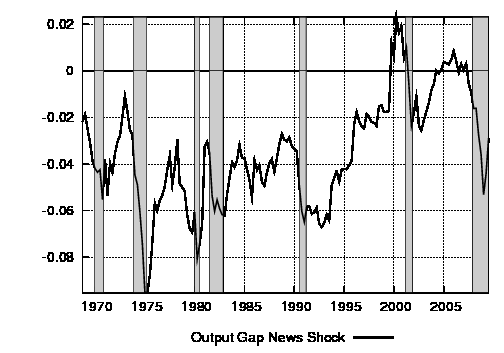
\includegraphics[scale=0.3]{yNewsShock.png} & 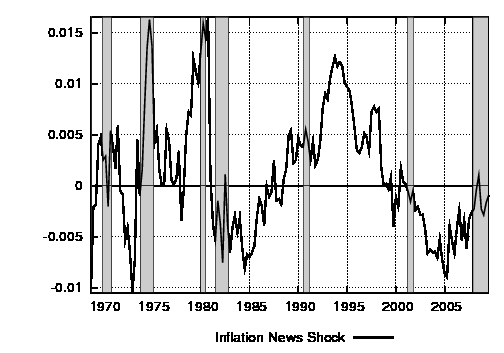
\includegraphics[scale=0.3]{piNewsShock.png} \\
  \end{tabular}
  \bi
  \item Negative shocks to output expectations precede each recession since 1970.
  \item Positive shocks to inflation expectations are associated with recessions in middle and late 1970s.
  \ei
}

\frame
{
  \ft{Structural Shocks}
  \hspace*{-0.2in}
  \begin{tabular}{cc}
    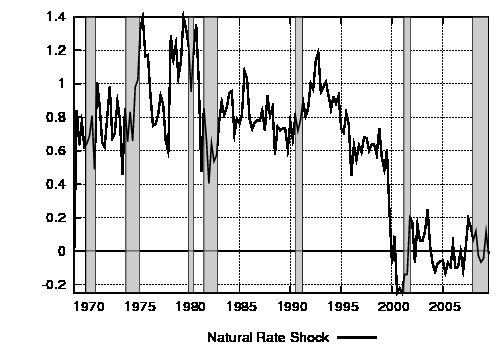
\includegraphics[scale=0.3]{natshock.png} & 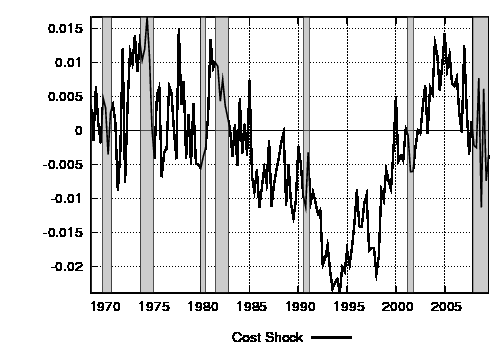
\includegraphics[scale=0.3]{costshock.png} \\
  \end{tabular}
  \bi
  \item Natural rate shock positive during most period.
  \item Fall in natural rate shock precedes the 2001 recession.
  \item Little change in volatility of shocks during ``Great Moderation''.
  \ei
}

\section{}
\subsection{Conclusion}
\frame
{
  \ft{Conclusions}
  \bi
  \item Findings:
    \bi
    \item Judgment is primarily determined by expectational shocks.
    \item Preliminary evidence suggests expectational shocks can be causing recessions.
    \item Preliminary evidence suggests expectational shocks Changes in macroeconomic volatility.
    \ei
  \item Next steps:
    \bi
    \item Impulse response functions to expectational shocks.
    \item Decomposition of forecast errors.
    \ei
  \ei
}


\end{document}

